\documentclass[12pt]{article}
\usepackage[utf8]{inputenc}
\usepackage{graphicx}
\usepackage{biblatex}
\usepackage{titlesec}
\usepackage{geometry}
\usepackage{setspace}
\usepackage{minted}
\usepackage{biblatex}
\usepackage{listings}

\geometry{
 a4paper,
 left=35mm,
 top=25mm,
 right=25mm,
 bottom=25mm,
 }
\setstretch{1.5}
\addbibresource{reference.bib}
\bibliography{reference}
\begin{document}
\graphicspath{{./pictures/}}
\titlelabel{\thetitle.\quad}
\renewcommand*\contentsname{Obsah}
\renewcommand{\bibfont}{\small}
\renewcommand{\thesection}{\Roman{section}} 
\renewcommand{\thesubsection}{\thesection.\Roman{subsection}}
\renewcommand{\thesubsubsection}{\thesubsection.\Roman{subsubsection}}
\renewcommand\listoflistingscaption{Seznam příloh}
\renewcommand{\listingscaption}{Příloha}
\begin{titlepage}
\begin{center}
    \vspace{2,5cm}
    \textbf{\Large Gymnázium, Praha 6, Arabská 14}\par
    \Large Obor Programování\par
    \vspace{2cm}
    \textbf{\Huge Ročníková práce}\par
    \vspace{2cm}
    \textbf{\Huge Custom Chess}\par
    \vspace{2cm}
    
\includegraphics[]{logo}\par
    \vfill
   \Large Petr Dobiáš, Josef Liška, Jakub Turek \hfill Duben 2023
   
    
     
\end{center}
\end{titlepage}
\newpage{}
\thispagestyle{empty}
\mbox{}
\vfill
Prohlašuji, že jsem jediným autorem tohoto projektu, všechny citace jsou řádně označené a všechna použitá literatura a další zdroje jsou v práci uvedené. Tímto dle zákona 121/2000 Sb. (tzv. Autorský zákon) ve znění pozdějších předpisů uděluji bezúplatně škole Gymnázium, Praha 6, Arabská 14
oprávnění k výkonu práva na rozmnožování díla (§ 13) a práva na sdělování díla veřejnosti (§ 18) na dobu časově neomezenou a bez omezení územního rozsahu.
\newline
V Praze dne \hfill Petr Dobiáš, Josef Liška, Jakub Turek
\newpage{}
\thispagestyle{empty}
\section*{Anotace}
Následující práce pojednává o vývoji aplikace založené na atchitektůře klient-server s využitím programovacích jazyku Java, Python a JavaScript, frameworku Django a databáze MongoDB, která umožnuje uživatelům vytvařet a následně hrát derivace hry šachy, v podobě úpravy figur, hrací desky a podmínek vítězství, online. Tyto derivace mohou uživatelé definovat ručně pomocí textovích soubru, či grafického návrháře v aplikaci. Aplikace se sestává ze serverové části a klientské webové aplikace.
\newpage
\setcounter{page}{1}
\tableofcontents 
\newpage
\section*{Úvod}
Následující práce pojednává o vývoji aplikace, jejímž cílem je umožnit uživatelům hrát v online multiplayeru derivace hry šachy a zároveň jim umožnit jednoduše tyto derivace vytvářet prostřednictvím grafického návrháře vlastních pravidel v klientské aplikaci. Přesná podoba těchto vlastních pravidel bude podrobněji rozebrána v následujících kapitolách, ale ve zkratce se jedná o možnost definovat vlastní rozměr šachovnice, rozložení figur nebo vytvoření vlastních figur a podobně.

Aplikace je založené na architektuře klient-server a skládá se tedy ze dvou částí. Serverové částí, která je napsaná v programovacím jazyku Java s využitím řady knihoven, kterým se budeme více věnovat později. A klientské části, kterou je v tomto případě webová aplikace, jejíž back-endová část je napsaná v jazyce Python s využitím frameworku Django, její front-endová část využívá CSS frameworku Bootstrap pro snazší práci s kaskádovými styly a JavaScriptové knihovny JQuery. Z tohoto důvodu bude tedy následující text rozdělen na dvě hlavní částy a to tedy na část pojednávající o serverové části aplikace a část pojednávající o klientské části aplikace.
\addcontentsline{toc}{section}{Úvod}
\newpage
\section{Tvorba vlastních pravidel hry šachy}
\newpage
\section{Server}
Následující kapitola pojednává o serverové části aplikace, tedy o její struktuře, technologiích použitých pro její vývoj, řešení některých klíčových problémů řešených v této části aplikace a také o komunikačním protokolu sloužícímu pro komunikaci mezi serverem a klientem.
\subsection{Použité technologie}
Následující kapitola poskytuje výčet technologií a knihoven používaných serverem a stručný popis jejich fungování a využití v tomto projektu
\subsubsection{MongoDB}
Jedná se on o NoSQL, což znamená, že místo klasické struktury tabulek známe z SQL databází, jsou data ukládána do souboru BSON, binární forma formátu JSON, což usnadňuje například ukládání souboru. Databázi je také možno v rámci služby Atlas provozovat v cloudu bez nutnosti vetší údržby, což je možnost, kterou využívá i tento projekt. Pro komunikaci s touto databází serverová část používat také MongoDB driver pro jazyk Java a také knihovnu Morphia, která poskytuje obdobu objektově orientovaného mapování pro NoSQL databázi MongoDB.
\subsubsection{Bouncy castel}
Jedná se o opensource knihovnu, která nabízí implementace většiny standartě používaných kryptografických algoritmů v jazyce Java\cite{bouncyCastle}. V tomto projektu je primárně využívána pro zabezpečení komunikace mezi klientem a serverem pomocí protokolu TLS 1.3, ale také pro bezpečné ukládání hesel do databáze ve standartu podporované Django frameworkem.
\subsubsection{Simple Java Mail a Jsoup}
Jedná se o knihovnu, která usnadňuje odesílání emailů pomocí Javy, kdy po prvotním nakonfigurování STMP serveru, případně dalších parametrů jako například šifrování zpráv, umožňuje jednoduše odesílat jak prosté textové zprávy, tak emaily definované pomocí HTML šablony. Právě druhá z možností je využívána v tomto projektu a pro dynamické vkládání dat, jako třeba url pro reset hesla, do HTML šablon je používána druhá ze zmíněných knihoven, HTML parser Jsoup. Obě tyto knihovny jsou tedy v tomto projektu využívány  pro odesílání emailu pro potvrzení registrace a případně reset hesla.
\subsubsection{Gson}
Knihovna vytvořená společností Google sloužící pro serializaci Java objektů do podoby textového řetězce ve formátu json. Slouží jednak pro načítání vlastních pravidel hry, která jsou uložena v několika souborech ve formátu json a také pro serializaci dat, které jsou během hry odesílaný serverem klientu pro zobrazení, jako aktuální rozložení figur a podobně.
\newpage
\subsection{Struktura aplikace a základy fungování}
Následující podkapitola se věnuje struktuře serverové aplikace a základním principům jejího fungování. Server je rozdělen na dva balíčky první z nich Connection, jak už název napovídá, se stará o síťovou komunikaci a autentizaci klientu, zatím co druhý balíček GameLogic, obstarává samotný průběh hry, tedy interpretaci vlastních pravidel hry a vyhodnocovaní tahů zahraných hráči. Následující dvě sekce, tedy stručně pojednávají o struktuře a fungování každého z těchto balíčků. 
\subsubsection{Connection}
Z hlediska funkce by se třídy tohoto balíčku dali rozdělit do pěti základních kategorií. Tyto kategorie a některé do nich spadající třídy budou zmíněny v následujícím stručném schnutí fungování aplikace, ale kompletní seznam tříd a jejich zařazení můžete najít v přiložené tabulce.

Po spuštění serveru dojde k načtení jeho konfigurace ze souboru \textit{config.json}, kde je specifikovaná, délka fronty, maximální počet připojených klientů, ale třeba také cesta k SSL certifikátu a privátnímu klíčí, který slouží pro zabezpečení komunikace, či STMP serveru pro odesílaní verifikačních emailu.

Poté je spuštěno hlavní vlákno serveru reprezentované třídou \textit{Server}, které je zodpovědné za navazování spojení s klientem a následné zařazení tohoto spojení buďto mezi obsluhované klienty, nebo, v případě překročení kapacity serveru, do fronty a také pomocné vlákno, reprezentované třídou \textit{}{QueueManager}, které je zodpovědné za správu fronty, tedy za odstraňování zavřených spojení z fronty, či zařazování spojení z fronty mezi obsluhovaná po uvolnění kapacity. Obě tyto třídy patří mezi vlákna režie, která jsou jak je již patrno za správu jednotlivcích spojení, či prostředků aplikace.

Pokud je na serveru ještě volná kapacita, dojde po zařazení spojení mezi obsluhovaná připojení je pro jeho obsluhu vytvořeno nové vlákno reprezentované třídou \textit{ClientThread} a je zahájena autentizační rutina, která neskončí dokud se uživatel úspěšně nepřihlásí nebo se nedojde k ukončení spojení. Pokud je autentizace úspěšně dokončena začne vlákno obsluhovat požadavky klienta, do doby dokud klient nevytvoří novou hru, nebo se nepřipojí do již existující hry. Protokol této komunikace bude popsán v další kapitole.

Ve chvíli kdy se uživatel připojí do hry, dojde k odeslání souboru potřebných pro danou hru, vlastní ikony figur, z databáze klientovi. Poté dojde k ukončení daného vlákna a komunikace začne být obsluhována vláknem reprezentovaným třídou \textit{GameThread}, které spravuje komunikaci mezi všemi hráči v jedné hře, hra probíhá na tahy, tudíž je žádoucí aby byli klienti obsluhování postupně. Vlákno \textit{GameThread} začne vyhodnocovat požadavky až po připojení všech hráčů. Třídy \textit{GameThread} a \textit{ClientThread} tedy patří mezi komunikační vlákna, jejich hlavním účelem je přijímat požadavky od klientu, spouštět příslušné metody pro jejich obsluhu a odesílání výsledků v podobě odpovědi.

Po záhejení hry už je pouze s pomocí tříd balíčku GameLogic v smyčce vyhodnocovány tahy jednotlivých hráčů a jsou jim vraceny jejich výsledky do doby, než je hra ukončena. V tuto chvíli je hráčum odeslán výsledek hry a \textit{GamesManager} odebere dohranou hru ze seznamu probíhajících her a komunikace s jednotlivými hráči je opět přesunuta do samostatných vláken.

Zbylé tři skupiny, o kterých jsem se v rámci popisu fungování balíčku nezmínil jsou třídy sloužící pro reprezentaci dat v databázi, které jsou používány pro objektově relační mapování dat v databázi. Třídy datových objektů, které jsou podobné předchozí skupině s tím rozdílem, že obsahují i data, které jsou potřeba pouze za běhu programu a není třeba je ukládat. Poslední skupinou jsou třídy s logikou, které obsahují pouze třídu \textit{Game}, která definuje průběh herní smyčky ve vlákně \textit{GameThread}.
\begin{listing}[!ht]
\begin{tabular}{ |p{3cm}|p{3,2cm}|p{3,2cm}|p{4cm}| }
\hline
\multicolumn{4}{|c|}{Rozaření tříd dle funkce} \\
\hline
 Vlákna režie& Pomocné třídy & Datové objekty & Databázová data \\
\hline
Server & Sender &Client &ClientDataObject\\
GamesManager & Reciever  & ServerParameters &  GameDataObject\\
\cline{3-3} QueueManager&EmailSender& Třídy s logikou & AuthenticationToken   \\
\cline{1-1} \cline{3-3} Komunikační vlákna & ParametersParser PasswordHasher & Game & FigureDataObject \\
\cline{1-1} ClientThread GameThread& SecureConnection Manager& &\\
& UserAuthenticator & &\\
\hline
\end{tabular}
\caption{Tabulka reprezentující rozřazení tříd balíčku Connection dle funkce}
\end{listing}
\
\newpage
\subsubsection{GameLogic}
\newpage
\subsection{Klíčové problémy a jejich řešení}
Následující kapitola pojednává o nejzásadnějších problémech, které bylo třeba na straně serveru vyřešit a popisuje jejich případné řešení.
\subsubsection{Komunikační protokol}
Jedním z klíčových problému aplikace bylo vytvořit efektivní a snadno použitelný systém komunikace mezi serverem a klientem. Pro tento účel jsem tedy vytvořili jednoduchý textový komunikační protokol, kdy se požadavek vždy skládá ze jména požadavku a jeho argumentů oddělených dvojtečkami. Následující ukázka kód tedy ukazuje vytvoření obecného požadavku a následně i konkrétní požadavek pro přihlášení. 
\begin{listing}[!ht]
\begin{minted}{python}
# obecný požadavek
request = 'rquest_name:arg1:arg2'
# příklad požadavku o autentikaci
# zjednodušeně znázorněné odeslání a přijetí dat
server_connection.send('signin:username:password') 
response = server_connection.reciece().split(':')
if(response[1] == 'success'):
    print('přihlášen')
else:
    print(response[1])  
\end{minted}
\caption{Ukázka vytvoření požadavku protokolu v jazyce Python}
\end{listing}
Jak je vidět z výše uvedeného příkladu, tak odpověď serveru na požadavek je v případě požadavku na provedení akce na serveru buďto \textit{msg:success} v případě úspěšného provedení,nebo \textit{err:error message} v případě selhání. Nebo v případě, že se jedná o požadavek o zaslání dat, zůstává chybová odpověd stejná, ale v případě úspěchu jsou navrácena požadovaná data ve formátu json.

Pro vysvětlení fungování protokolu následující tabulka uvádí všechny možné požadavky, seznam jejich argumentů (je třeba je zadat v uvedeném pořadí) a typ jejich odpovědi.
\newpage
\begin{listing}[!ht]
\begin{tabular}{ |p{4cm}|p{6cm}|p{4cm}| }
\hline
název požadavku & argumenty & návratová hodnota \\
\hline
signin & username, password & None \\
signup & username, password, email & None\\
reset & username/email & None\\
crtg & game name, password, rules name & None\\
joig & game name, password & array of images \\
getg & None & array of games names\\
getr & None & array of rules names\\
\hline
\end{tabular}
\caption{Seznam všech požadavků a jejich argumentů}
\end{listing}
\subsubsection{Znovu připojení do hry}
Další zásadní problémem byla nutnost vyřešit způsob, jak umožnit hráči, který v době kdy se účastní hry ztratí spojení se serverem, znovu se připojit do rozehrané hry a dohrát ji.

Řešení tohoto problému se nakonec ukázalo jako ne tak komplikované, jak by se na první pohled mohlo zdát. Pro implementaci této mechaniky totiž stačí používat unikátní identifikátory pro každé připojení do hry, které jsou v našem případě reprezentovány náhodným textovým řetězcem.

Vzhledem k tomu, že běžící server si uchovává informace o připojených klientech ve formě instancí třídy \textit{Client}, je možné vždy při připojení do nové hry do této instance uložit, náhodně vygenerovaný textový řetězec, jeho generování je znázorněno v ukázce níže, a zároveň tento identifikátor uložit pro daného uživatele do databáze.

\begin{listing}[!ht]
\begin{minted}{java}
 private String getRandomString(int size) {
        byte[] stringBytes = new byte[size];
        new Random().nextBytes(stringBytes);
        return new String(Base64.encodeBase64(stringBytes));
}
\end{minted}
\caption{Generování náhodného řetězce v jazyce Java}
\end{listing}

Po implementování těchto identifikátorů už jen stačí pokaždé, když je navázáno nové spojení s klientem získat z databáze tento identifikátor, a pokud se shoduje s identifikátorem některého z odpojených hráčů, jednoduše spoji toto nové připojení s daty o daném hráči.

Poté už stačí jen kdykoliv, kdy dojde ke ztrátě spojení, místo ukončení hry pouze označit daného hráče za odpojeného a spustit timeout po jehož vypršení dojde ke kontrole zda se daný hráč znovu připojil a pokud ano, je mu odeslán aktuální stav hry a hra pokračuje, v opačném případě je hra ukončena.
\subsubsection{Autentizace klientů}
Dalším ze zásadních problémů bylo při spuštění ověřit identitu uživatele a zobrazit mu pouze jemu náležící data, a tedy v podstatě vytvořit uživatelské účty.

Vyřešit tento problém nebylo zdaleka tak náročné, jelikož se jedná o jeden z nejčastěji řešených problémů a je jeho řešení je tedy velmi dobře zdokumentované a má jasně formulované postupy dobré praxe, kterých se držet pro vytvoření bezpečných uživatelských účtů. Tento projekt využívá pro ukládání hesel standard užívaného frameworkem Django\cite{djangoJava}\cite{djangoPassword} a to z důvodu snazšího procesu změny hesla, která je dokončována právě webovou aplikací napsanou s pomocí Django frameworku. Nyní tedy přejděme k samotnému procesu vytvoření uživatelského účtu.

Poté, co uživatel zašle požadavek o vytvoření nového účtu, dojde k ověření zda-li pro zadaný email a jméno již účet neexistuje a pokud ne, jsou zadané údaje uloženy do databáze jakožto nový uživatelský účet, který ale zatím není aktivovaný a nemůže se pomocí něj nikdo přihlásit. Proto aby byl účet aktivován, je nejprve nutné ověřit zadaný email, pomocí odkazu, který byl na tento email zaslán\cite{email}. Tento odkaz vede na webovou aplikaci, která se stará o ověřování uživatelských účtu a jako base64 je v něm zakódované id daného uživatele a hodnota autentizačního tokenu, který je vygenerován\cite{tokenCreate} při vytvoření účtu a tvoří ho hodnota, kterou představuje náhodný řetěze, který je generován jako v předchozím případě akorát s využitím kryptograficky bezpečného náhodného čísla a data expirace, které je nastaveno na den po vygenerování. Hash jeho hodnoty a datum expirace je uloženo pro daný účet do databáze. Po otevření zaslané adresy z ní tedy webová aplikace získá id uživatele a hodnotu autentizačního tokenu, následně tedy spočítá hash získané hodnoty a zjistí zdali je pro uživatele s daným id v databázi uložený platný token hash jehož hodnoty by odpovídal vypočítanému hashy\cite{token}, pokud ano je účet aktivován, token odstraněn z databáze a uživatel se může přihlásit, v opačném případě se mu zobrazí chybová hláška a účet zůstane neaktivní.

Pokud se uživatel přihlašuje pomocí již existujícího účtu, je na server poslán požadavek, který obsahuje uživatelem zadané uživatelské jméno, nebo email a heslo. V tomto případě je v databázi jednoduše vyhledán uživatel s daným emailem, nebo jménem a jsou získány informace s jakým algoritmem, saltem a počtem iterací byl vypočítán hash\cite{passwordHash} jeho hesla uložený v databázi a s pomocí těchto údajů je vypočítán hash hesla zaslaného v požadavku, pak už stačí oba hashe porovnat a v případě, že se shodují je uživatel přihlášen.

Pokud uživatel zažádá o změnu hesla, je průběh téměř totožný aktivaci nového účtu, s tím rozdílem, že po úspěšném ověření webová aplikace uživatele vyzve k zadání nového hesla, vygeneruje pro něj nový salt a s jeho pomocí spočítá hash nového hesla, tyto informace jsou následně uloženy do databáze a uživatel se může přihlást pomocí nového hesla. 

\subsubsection{Ukládání dat do databáze}
Jedním z posledních problémů, které bylo třeba vyřešit, bylo jak reprezentovat uživatelská dat v databázi. Pro demonstraci toho, jaká data jsou v databázi uloženy a jaké jsou mezi nimi vztahy, slouží následující schema, pro jehož použití jsem se rozhodl, i přesto že MongoDB nemá na rozdíl od SQL databází nic jako fixní schéma, ale považoval jsem ho za vhodnější formu popisu uložených dat než slovní popis, zároveň bych chtěl ještě dodat, že pole souborů by samozřejmě opět šlo rozepsat jako one-to-many relation mezi výchozí kolekcí a kolekcí file, ale vzhledem k tomu, že kolekce file je vytvářena samotnou databází, rozhodl jsem se použít toto zjednodušení.
\begin{listing}[!ht]
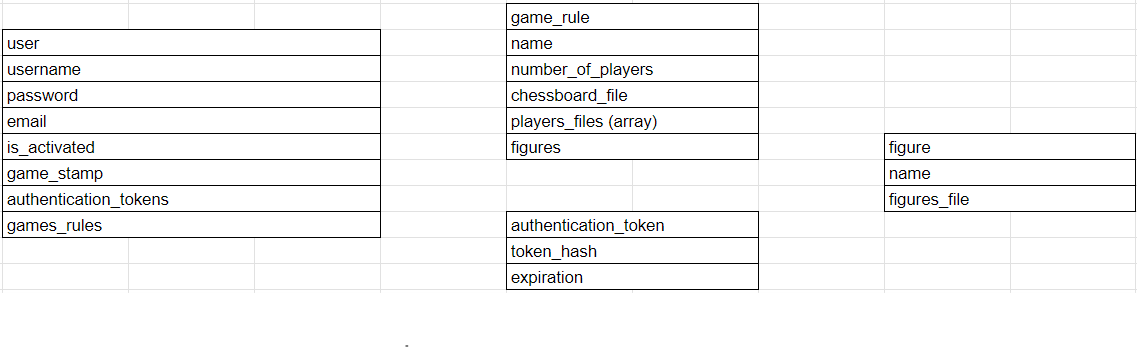
\includegraphics[scale=0.75, width=15cm]{pictures/schem.png}\par
\caption{Schéma databáze}
\end{listing}
\newpage
\section{Klient}
Následující část pojednává o klientské části aplikace a bude strukturována podobně jako předchozí část o serveru, tedy v krátkosti zmíní použité technologie a jejich využití v projektu, následně nastíní strukturu a fungování aplikace a na závěr popíše hlavní problémy řešené v klientské aplikaci a jejich řešení.
\subsection{Použité technologie}
Následující podkapitola stručně poskytuje stručný výčet všech hlavních technologií použitých v aplikaci a ve zkratce popisuje jejich využití.
\subsubsection{Django}
Django je webový framework založený na architektůře model-view-controller nepsaný v jazyce Python, který nabízí například dynamické vkládání dat do html šablon, či vlastní mapper pro snadnou práci s databází. 
\subsubsection{Django channels}
Django channels je projekt, který rozšiřuje možnosti frameworku Django o podporu i dalších protokolu něž je pouze HTTP, jako třeba WebSocket a IoT protokoly a zároveň umožňuje také asynchronní odbavování příchozích požadavků\cite{channels}. V tomto projektu jsou tento projekt využíván primárně pro implementaci komunikace prostřednictvím protokolu WebSocket\cite{webSocket}.
\subsubsection{Djongo}
Djongo je projekt, který zase Django framework Django rozšiřuje po stránce práce s databází, kdy poskytuje právě již výše zmíněný mapper pro databázi MongoDB, který tak umožňuje využití této databáze bez nutnosti měnit kód napsaný pro výchozí mapper Django frameworku, který podporuje pouze SQL databáze\cite{djongo}.
\subsubsection{Bootstrap}
Je framework, který nabízí mnoho již před vytvořených komponent pro snadné a rychlé, ale v porovnání s konkurencí zároveň poměrně špatně přizpůsobitelné, navrhování designu webových aplikací\cite{bootstrap}. V rámci tohoto projektu je využit pro design šablon Django frameworku.
\subsubsection{Cropper js}
Cropper js je jednoduchá JavaScriptová knihovna, které umožňuje snadné snadné ořezávání obrázků na straně klienta\cite{cropperGit}. Knihovna poskytuje již hotovou komponentu crroperu, které stačí nastavit zdroj obrázku a ona posléze nechá uživatele prostřednictvím grafického rozhraní vybrat oblast k oříznutí a poté vrátí daný výřez, který je možné dále zpracovat\cite{cropperImp}.
\subsubsection{JQuery}
JQuery je JavaScriptová knihovna, která zjednodušuje interakci mezi JavaScriptem a HTML a zároveň také zjednodušuje syntaxi provádění některých funkcí, jako je například vytváření AJAX požadavků\cite{JQuery}, což je také hlavní spolu se zmíněnou interakcí s HTML hlavním využitím JQuery v tomto projektu.
\newpage
\subsection{Struktura aplikace a základy fungování}
Tato kapitola se zaobírá obecnými principy fungování klientské aplikace a její strukturou, která je vzhledem k tomu, že slouží v podstatě pouze ke komunikaci se serverem a zobrazovaní jeho odpovědí uživateli, podstatně jednodušší než struktura serveru.

Struktura samotné ho projektu se příliš neliší od běžné struktury projektu využívajícího frameworku Django. Projekt se skládá ze dvou aplikací, což je termín používaný Djangem pro znovu použitelné komponenty, a to konkrétně z aplikace \textit{Game}, která reprezentuje část aplikace se samotnou hrou a aplikace \textit{Verification}, která se stará ověřování uživatelských účtu a změnu hesel k nim. Nyní si tedy přejděme k popisu těchto dvou celků.

Aplikace \textit{Verification}, je velmi jednoduchá a skládá se celkem pouze ze čtyř stránek (stránka pro ověření emailů, změnu hesla, úspěšné provedení operace a chybová stránka), na které se dá v případě prvních dvou dostat pouze s platný odkazem vygenerovaným serverem a na zbyle dvě musí být klient přesměrován serverem po provedení jedné z akcí\cite{redirect}. V případě, že se uživatel pokusí tyto stránky navštívit, jinak než legitimní cestou přes ověřovací odkaz je mu vrácena HTTP 403 response s custom chybovou stránkou. Myslím, že o fungování back-endu této aplikace není třeba se zde více zmiňovat, jelikož je poměrně podrobně popsáno v předchozí části v sekci autentizace klientů.

Aplikace \textit{Game} je o poznání rozsáhlejší a na rozdíl od aplikace \textit{Verification} je zde i pozměněna struktura od klasického Django projektu kvůli použití WebSocket protokolu s využitím Django Channels, které do této aplikace přidávají soubory \textit{consumers.py} a \textit{routing.py}, které jsou obdobou klasicky používaných \textit{views.py} a \textit{urls.py} pro HTTP protokol akorát pro protokol WebSocket. Jak \textit{consumers.py} tak \textit{urls.py} používají funkcionální přístup, což je výchozí forma používaná Djangem, ale liší se od zbytku projektu, který používá objektové paradigma.

Dalé se na back-endu nachází třída \textit{Connection}, která používá návrhový vzor singelton a reprezentuje spojení se serverema implementuje metody pro zapisovaní a čtení dat z tohoto spojení. Tato třída je také úzce spojená s pomocným vláknem, které je spuštěno vždy, když hráč není na tahu a stará se o přijímání dat ze serveru a s pomocí WebSocketu odesílá požadavky na jejich vykreslení na front-endu, tato problematika ale bude podrobněji popsána později.

Nyní se tedy přesuňme k front-endu aplikace. Django framework mimo jiné umožňuje dědičnost mezi jednotlivými šablonami, což umožňuje jejich rychle a efektivní vytváření, jelikož nemusíme znovu psát jejich opakující se části. Této funkce je v tomto projektu hojně využíváno a pro účely jejího použití je zde vytvořena šablona \textit{base.html}, která sice nikdy není zobrazena uživateli, ale obsahuje elementy opakující se na všech stránkách jako navigační menu, mini profil uživatele a podobně, a všechny ostatní šablony je z ní dědí a pouze do ní vkládají pro ně unikátní elementy, jako šachovnice, formulář pro přihlášení a podobně, což umožňuje minimalizovat množství HTML napsaného při vytváření šablon.

Aplikace má celkem pět stránek (úvodní stránka, registrace, připojení do hry, vytvoření hry a hra samotná), pro stránky registrace, pripojení do hry, vytvoření nové hry a stránku se hrou existuje ještě separátní soubor s JavaScriptem, pouzev případě stránek pro připojení do hry a vytvoření nové hry, které jsou si na tolik podobné, že sdílí stejný JavaScript. Tyto soubory s JavaScriptem s starají o responzivitu stránek, odesílání dat back-endu, či vyhledávání ve zobrazených datech\cite{search}. Některé ze zajímavějších problému, které jsou s jeho pomocí řešeny budou ještě podrobněji popsány v další kapitole.
\newpage
\subsection{Klíčové problémy a jejich řešení}
Následující sekce uvádí některé ze zásadních problémů řešených v klientu a popisuje jejich řešení.
\subsubsection{Responzivní šachovnice}
Jedním z prvních problému, který bylo potřeba vyřešit bylo, jak vlastně zobrazit samotnou šachovnici. Pro tento účel se zdál jako ideální HTML element \textit{canvas}, který ovšem má pro nás dva zásadní problémy a to za prvé, že jeden canvas nemůže mít více vrstev, což je v tomto případě problematické, z důvodu animací, kdy by s každým snímkem animace pohybující se figury musel být překreslen kus pozadí a zároveň tagy, které zobrazují další stav daného políčka a za druhé, že canvas není ze své podstaty responziví a je tedy nutné ho při každé změně velikosti okna manuálně resizovat a překreslit v novém měřítku. Nyní tedy přejděme k řešení těchto problémů.

Asi nejsnazším řešením prvního z problémů bylo reprezentovat každou vrstvu šachovnice, tedy vrstvu pozadí, tagů, figur, vrstvu pro zobrazení možných pohybů figury a vrstvu pro animace, jako několik canvasů s absolutní pozicí na sobě, zabalené do elementu \textit{div}, který bude mít relativní pozici a bude pozici šachovnice přizpůsobovat okolním elementům. To jak vypadá výsledná komponenta reprezentující šachovnici můžete vidět na následující ukázce.

\begin{listing}[!ht]
\begin{minted}{html}
 <div id="chessboard" style="position: relative;">
   <canvas style="position: absolute; z-index: 0"></canvas>
   <canvas style="position: absolute; z-index: 1"></canvas>
   <canvas style="position: absolute; z-index: 2"></canvas>
   <canvas style="position: absolute; z-index: 3"></canvas>
 </div>
\end{minted}
\caption{HTML komponenta reprezentující šachovnici}
\end{listing}

Druhý z problému je řešen, tak že data potřebná pro vykreslení šachovnice, která jsou předána serverem při načtení stránky a jsou průběžně aktualizovány s každým tahem, jsou uložena JavaScriptu zodpovědném za obsluhu dané stránky a pokaždé, když dojde ke změně velikosti okna, je zavolána funkce, která nejprve spočítá nový rozměr jednoho políčka šachovnice, podle vzorce, kdy minimum z podílu výšky okna a počtu políček šachovnice ve vertikálním směru a šířky okna a počtu políček v horizontálním směru, a poté změní rozměr canvasů na součin počtu políček v daném směru a tohot nově získaného rozměru a nakonec jsou opět zavolány funkce zodpovědné za vykreslení jednotlivých vrstev, které vrstvy překreslí,tak aby odpovídaly novým rozměrům.

\subsubsection{Animace s vlastními ikonami figur}
Z hlediska animací nebylo až takovým problémem provádění samotných animací, jelikož JavaScript poskytuje funkci \textit{drawAnimationFrame()}, která asynchronně vykreslí jeden snímek animace a je možné jí rekuzivně volat až do dokončení celé animace a jelikož všechny pohyby prováděné v rámci animací jsou pohyby po přímce mezi dvěma body, jedná se při výpočtu nové pozice, na které má být daný snímek animace vykreslen, pouze o aplikaci obecné rovnice přímky, pomocí které je vždy nalezena nová pozice figury na daném snímku, dokud se figura nedostane na cílovou pozici.

Větším problémem bylo vzhledem k tomu, jak moc je tento projekt založen na uživateli vytvořeném obsahu, namapování jmen hráči vytvořených figur ke správným ikonám, které pro ně hráči nahráli. Tento problém je vyřešen pomocí slovníku, který je klientu poslán ve chvíli kdy se připojí do hry, společně s dočasnými soubory, tedy ikonami vlastních figur, a obsahuje dvojici hodnot, kdy klíč je jméno vlastní figury a hodnota je název příslušného dočasného souboru, který má být použit jako ikona. Poté už tedy stačí se pouze ve chvíli, kdy dochází k vykreslování figur, získat dat o stavu šachovnice vráceného serverem jméno figury a následně se pomocí slovníku dotázat na konkrétní soubor.
\subsubsection{Zobrazení akcí ostatních hráčů}
Posledním větším problémem, který bylo třeba vyřešit bylo zobrazení akcí provedených ostatními hráči připojenými ke stejné hře. Jak už bylo zmíněno výše pro řešení tohoto problému je využíváno WebSocket protokolu a na něm postaveném velmi jednoduchém textovém komunikačním protokolu.

Požadavek je v tomto protokolu reprezentován slovníkem serializovaného do formátu json a může mít pouze dva typy \textit{join} a \textit{move}. První z požadavků slouží pro přidání hráče do seznamu připojených hráčů a má pouze jeden parametr a to \textit{username}, který reprezentuje jméno připojeného hráče. Druhý z požadavků slouží pro zobrazení tahu jiného hráče, a má dva parametry \textit{cordinates}, který je tvořen čtyřmi čísly oddělenými dvojtečkami, které představuji souřadnice počátečního a koncového bodu animace tahu a parametr \textit{figure}, který představuje typ figury se kterou má být animace provedena.

Jak už bylo zmíněno na straně back-endu je tento problém řesen pomocí vlákna, které přijímá data ze serveru a na jejich základě posílá prostřednictvím WebSocketu příslušné požadavky front-endu.

JavaScript na straně front-endu pak jenom otevře připojení přes WebSocket s back-endem a čeká na chvíli, kdy jeho prostřednictvím přijde zpráva, ve chvíli kdy se tak stane, serializuje ze zprávy slovník a na zákldě parametru \textit{type} rozhodne zda má dojít k vykreslení příslušné animace, nebo zda má být přidána nová karta hráče do seznamu aktivních hráčů.
\newpage
\section{Instalace}
Proto aby bylo aplikaci možné v budoucnu používat by neměla být nutná žádná instalace, bude jednoduše stačit otevřít v prohlížeči doménu, na které bude hostován webový klient a hrát, bohužel v současné chvíli není projekt nikde nasazen. Pro případ, že byste si chtěli aplikaci nasadit sami postupujte podle následujícího návodu.

Instalace serveru je velmi jednoduchá, pro jeho spuštění stačí mít na zařízení, na které ho chcete nainstalovat, Javu 16 a vyšší, jelikož u starších verzí dochází k problémům při komunikaci s databází, a také získat SSL certifikát pro danou ip adresu, ten můžete bezplatně získat třeba pomocí služby ZeroSSL, kde stačí postupovat podle návod na jejich webových stránkách. Ve chvíli, kdy máte tyto věci připraveny, už stačí pouze na vašem zařízení rozbalit obsah složky dist tohoto repozitáře a ve složce AppData v souboru \textit{config.json} nakonfigurovat, cestu k certifikátu a klíčí, který jste získali od certifikační autority, connection string pro MongoDB databázi (doporučujeme využít free tier služby Atlas) a informace o email, který chcete používat pro zasílání ověřovacích emailu (v tuto chvíli jsou podporovány pouze emailu služby Gmail). Po tomto nastavení už stačí spustit spustitelný soubor \textit{ChessServer.jar} a server by se měl spustit.

V případě klientu je situace obdobná, akorát v konfiguračním souboru stačí vyplnit pouze cestu k důvěryhodnému kořenovému certifikátu certifikační autority, ip adresu serveru a connection string k databázi. Následně, vzhledem k tomu, že nasazení ASGI Django projektu není úplně triviální, doporučuji postupovat podle online dostupných návodů, které danou problematiku vysvětlují lépe, než jsem tomu na tomto místě schopen učinit\cite{deployment}.

V případě, že si chcete aplikaci pouze vyzkoušet na localhostu, je postup v případě serveru téměř stejný, pouze můžete použít selfsigned SSL certifikát, místo reálného certifikátu od certifikační autority. A v případě klientu je postup podstatně jednodušší, kdy konfigurační soubor vyplníte stejně jako v předchozím případě, akorát můžete za důvěryhodný certifikát použít ten, kterým se prokazuje server. Poté už stačí si jen vytvořit Python virtual enviroment, nainstalovat požadavky ze souboru \textit{requirements.txt} a následně zinicializovat databázi pomocí dvojice příkazů \textit{py manage.py makemigrations} a \textit{py manage.py migrate} a následně aplikaci spustit pomocí \textit{py manage.py runserver}
\newpage
\section{Závěr}
Nyní přejděme k závěrečnému zhodnocení celého projektu a případným návrhům na jeho vylepšení, kterými by mohl v budoucnosti projít.

Osobně bych celý projekt hodnotil jako částečně úspěšný, jelikož se nám podařilo vytvořit poměrně robustní komunikační infrastrukturu a většinu algoritmů potřebných pro vyhodnocování vlastních pravidel, avšak nepodařilo se nám dostát cíli vytvořit například i desktopovou verzi klientské aplikace, kterou jsme se nakonec rozhodli upozadit na úkor více univerzální webové aplikace. A celkově mé aplikace stále ještě mnoho nedostatků a to zejména v oblasti tvorby uživatelského obsahu, který by měl být její hlavní náplní, a oblasti celkové stability a celkově je spíše ve stavu konceptu, nežli funkčního řešení.

Do budoucna bychom tedy chtěli vylepšit hlavně tvorbu uživatelského obsahu a celkovou stabilitu aplikace a také samozřejmě po odstranění těchto problémů aplikaci nasadit do produkce a zpřístupnit ji uživatelům.

\newpage
\printbibliography[heading=bibintoc,title={Reference}]
\newpage
\addcontentsline{toc}{section}{Seznam příloh}
\listoflistings


\end{document}
